\section{Results}

Two stages of results were evaluated:
\begin{enumerate}
\item Result of the depth map estimated by the neural network
\item Performance of the overall path planning control policy
\end{enumerate}

\begin{figure}
  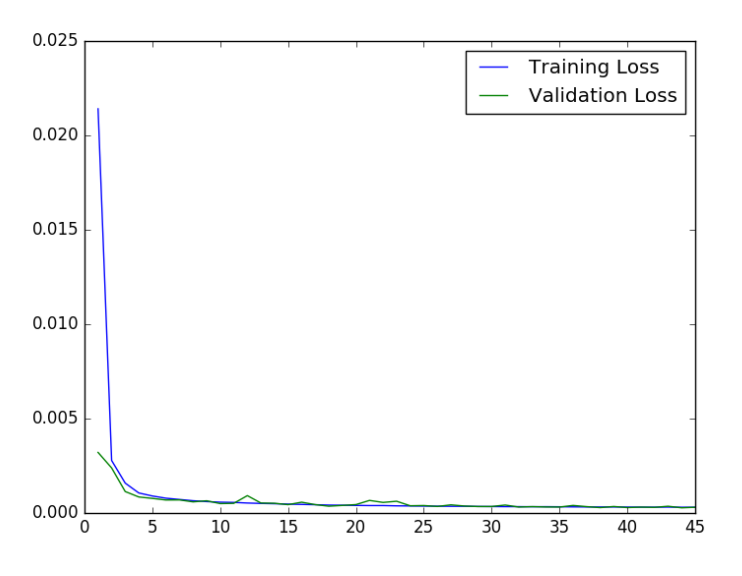
\includegraphics[width=\linewidth]{images/validationloss.png}
  \caption{Training and Validation loss of depth map}
  \label{fig:boat1}
\end{figure}

The neural network was able to accurately estimate the depth parity given 2 input stereo images. The validation loss was calculated by comparing the ground truth depth information against the predicted depth map obtained from the neural network.

Validation loss was determined to be in the order of 10-3 . 

\begin{figure}
  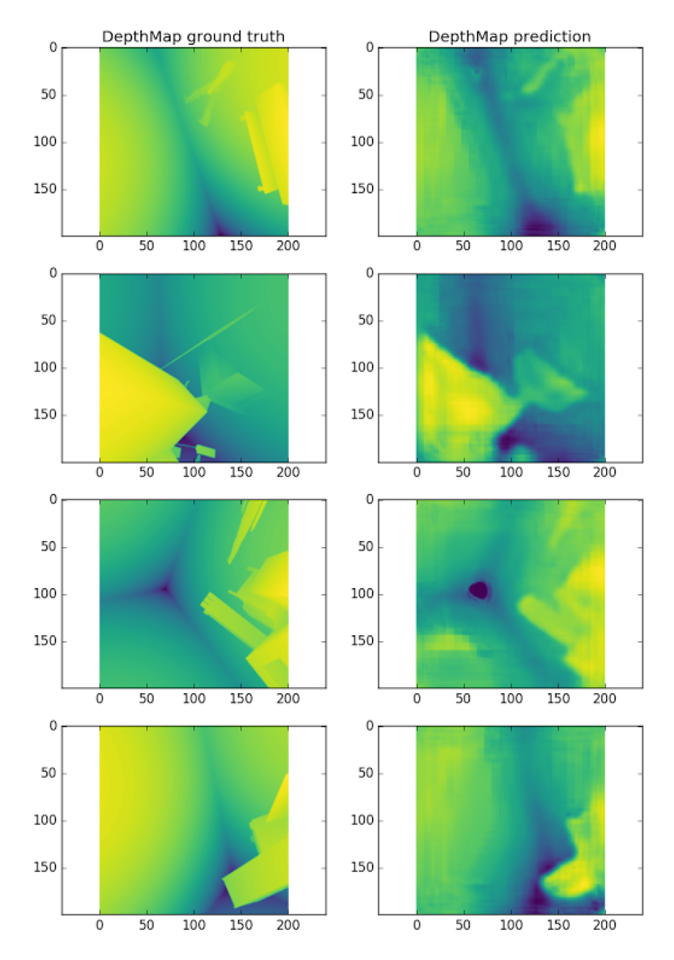
\includegraphics[width=\linewidth]{images/depthmap2.png}
  \caption{Performance of depth map on simulated images}
  \label{fig:depthmap2}
\end{figure}

The performance of the algorithm with different heuristics is stated in the following table below.
 
S No. = Scenario number of experiment, with each scenario having different source and destination points
MManhattan : The step count of the control policy using Manhattan distance as base distance heuristic.
 
MEuclidean : The step count of the control policy using Euclidean distance as base distance heuristic.
 
Human Benchmark : The step count of a human performing the experiment
 
Relative MManhattan : The ratio of MEuclidean to Human Benchmark performance (Lower is Better)
 
Relative MEuclidean : The ratio of MEuclidean to Human Benchmark performance (Lower is Better)

\begin{table}[h!]
  \centering
  \caption{Caption for the table.}
  \label{tab:table1}
  \begin{tabular}{cccccc}
    \toprule
      S No. & Baseline & M & M  & Rel & Rel\\
    \midrule
    	1 & 179 & 330 & 241 & 1.84 & 1.35\\
    	2 & 209 & 472 & 472 & 2.26 & 2.26\\
    	3 & 276 & 556 & 520 & 2.01 & 1.88\\
    	4 & 269 & 252 & 551 & 0.93 & 2.05\\
    	5 & 167 & 401 & 401 & 2.40 & 2.40\\
    	6 & 197 & 462 & 361 & 2.35 & 1.83\\
    	7 & 123 & 114 & 114 & 0.93 & 0.93\\
    \bottomrule
  \end{tabular}
\end{table}


The average relative performance of the Manhattan based heuristic was found to be 1.81
The median relative performance of the Manhattan based heuristic was found to be 2.01
The average relative performance of the Euclidean based heuristic was found to be 1.80
The median relative performance of the Euclidean based heuristic was found to be 1.88
 
Despite the comparable measures of the average relative performance, the average is susceptible to outliers in the observations, hence the median is a better measure of the relative performance of the heuristics.
  
The Euclidean heuristic equaled or outperformed the Manhattan heuristic on 85.71\% of the experiments, and is hence a better heuristic for evaluation.


\begin{figure}
  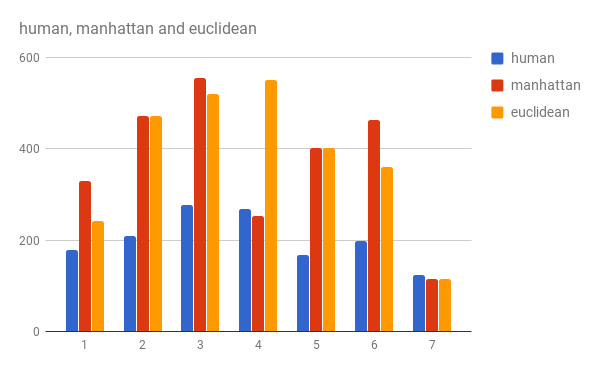
\includegraphics[width=\linewidth]{images/chart.png}
  \caption{Performance of heuristics vs humans}
  \label{fig:chart1}
\end{figure}